% Data flow diagram
% Author: David Fokkema
\documentclass{article}
\usepackage{tikz}
\usetikzlibrary{shapes,arrows}
\usepackage{pdflscape}
\usepackage[papersize={8.9cm, 2.8cm}, text={8.9cm, 3.5cm}]{geometry}
\usetikzlibrary{decorations.text}
\usepackage{xcolor}
% \selectcolormodel{gray}

\begin{document}
\thispagestyle{empty}
%\begin{landscape}
\begin{center}
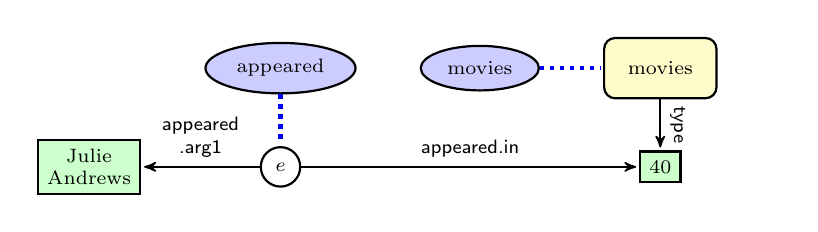
\begin{tikzpicture}[
  font=\sffamily,
  every matrix/.style={ampersand replacement=\&,column sep=0.8cm,row
sep=0.5cm,font=\scriptsize},
  entity/.style={draw,thick,rectangle,fill=green!20,font=\scriptsize},
  word/.style={draw,thick,ellipse,fill=blue!20},
  mediator/.style={draw,thick,circle},
  entityType/.style={draw,thick,rounded corners,fill=yellow!20,inner sep=.3cm},
  mathType/.style={draw,thick,diamond,fill=red!20},
  mediatorToEntity/.style={->,>=stealth',shorten
>=1pt,semithick,black,sloped,above,font=\sffamily\scriptsize},
  typeToEntity/.style={->,>=stealth',shorten
>=1pt,semithick,black,sloped,above,font=\sffamily\scriptsize},
  wordToEntity/.style={-,>=stealth',shorten >=1pt,ultra
thick,dotted,blue,sloped,above,font=\sffamily\scriptsize},
  entityToMath/.style={->,>=stealth',shorten >=1pt,ultra
thick,dashed,violet,sloped,above,font=\sffamily\scriptsize},
  every node/.style={align=center}]

  % JulieAndrews has appeared in 40 movies .
  
  % Position the nodes using a matrix layout
  \matrix{ 
     \& \node[word] (wAppeared) {appeared}; \&
\node[word]
(wMovies) {movies}; \& \node[entityType] (tMovies) {movies}; \& \\
    \node[entity] (eAndrews) {Julie\\Andrews}; \& \node[mediator]
(mAppeared) {$e$}; \& \& \node[entity] (e40) {40};\\
  };
 
  % words to entities
  % \draw [wordToEntity] (wAndrews) edge node {}  (eAndrews);
  % \draw [wordToEntity] (w40) edge node {}  (e40);
  % words to types
  \draw [wordToEntity] (wMovies) edge node {}  (tMovies);
  % event word to mediators
  \draw [wordToEntity] (wAppeared) edge node {}  (mAppeared);
  
  % mediator to entities
  \draw [mediatorToEntity] (mAppeared) edge node {appeared\\.arg1} 
(eAndrews);
  \draw [mediatorToEntity] (mAppeared) edge node {appeared.in}  (e40);
  
  % types to entities
  \draw [typeToEntity] (tMovies) edge node {type}  (e40);
  
  % math func
  % \draw [entityToMath] (eMovies) edge node {}  (mMovies);
  % \draw [entityToMath] (mMovies) edge node {}  (e40);
  
  
  
\end{tikzpicture} 
\scriptsize $\mbox{appeared.arg1}(e, \mathrm{Julie Andrews}) \wedge
\mbox{appeared.in}(e, 40) \wedge \mbox{movies}(40)$
\end{center}

% \end{landscape}

% \begin{tikzpicture}
% \node (One) at (-3,0) [shape=circle,draw] {$One$}; 
% \node (Two) at (3,0) [shape=circle,draw] {$Two$};
% \def\myshift#1{\raisebox{-2.5ex}}
% \draw [->,thick,postaction={decorate,decoration={text along path,text
%align=center,text={|\sffamily\myshift|Some more bent text}}}] (One) to [bend right=45]  (Two);
% \def\myshift#1{\raisebox{1ex}}
% \draw [->,thick,postaction={decorate,decoration={text along path,text
%align=center,text={|\sffamily\myshift|Some bent text}}}]      (One) to [bend left=45] (Two);
% \end{tikzpicture}


\end{document}